\documentclass[../main.tex]{subfiles}
\begin{document}
\graphicspath{{figures/}{task5/figures/}}

\subsection{Task 5: Account Security Monitoring (unsupervised F3)}
\label{sec:t5}

\subsubsection{Problem and Data}

Task 5 asks for an unsupervised detector of anomalous player accounts: account takeovers, account-selling rings, bot farms, VPN abusers and other unusual behaviour. The course brief describes a security team that is flooded with alerts (a rule-based system with a 60\% false positive rate, more than 5,000 confirmed account thefts per month) and asks for a system that learns normal behaviour without labels. The data contain \textbf{25,889 test accounts, no training set and no labels}. Every design decision therefore comes from the structure of the test file itself, and no model can be fitted or validated against a ground truth.

Each account has 123 columns: 29 behavioural metrics recorded in four periods (suffixes \texttt{\_1} to \texttt{\_4}, 116 columns, for example \feat{login_count}, \feat{kda_std}, \feat{login_lat}), the static columns \feat{account_age_days} and \feat{behavior_stability}, four security-related flags (\feat{password_changed}, \feat{vpn_usage}, \feat{suspicious_login_time}, \feat{mass_item_sale}), and \feat{player_id}. About 4.84\% of all cells are missing, and \feat{behavior_stability} is missing in 4.86\% of accounts. The organisers re-released the data on 12 November; every number in this section comes from the new release.

\paragraph{Metric.} The score is the binary F3 of the anomaly class, $F_3 = \dfrac{10\,TP}{10\,TP + 9\,FN + FP}$. A missed anomaly costs nine times as much as a false alarm. If we add one account with probability $p$ of being anomalous to the flagged set, the expected $F_3$ rises exactly when $p > F_3/10$. At the scores we reach (about 0.997) this break-even is $p^\ast \approx 10\%$, a much lower bar than for an ordinary classifier; we use it for the final recovery step (Section~\ref{sec:t5-model}). Probes on the public leaderboard showed that Task 5 carries a weight of about 0.2 of the final score: submitting an all-zero Task 5 column cost $-0.177$.

\subsubsection{EDA Findings}

Without labels, EDA is the model. We ask one question of every view of the data: is there a population separated from the normal bulk by an empty gap, a break in time, or a joint box? The data are synthetic, so we expected normal accounts to be generated with near-independent features and each anomaly type to be injected by an explicit mechanism that breaks that independence.

\paragraph{Sudden breaks between periods.} Takeovers should show up as a change between the first two periods (the account's baseline) and the last two. For each account we measured the largest distance of the period-3/4 login coordinates from the home position (mean of periods 1 and 2) and, for every metric, the robust $z$-score (median and MAD) of the period-3/4 change. We then took the second-largest $z$ across metrics so that one noisy metric cannot trigger the rule.

\begin{figure}[H]
\centering
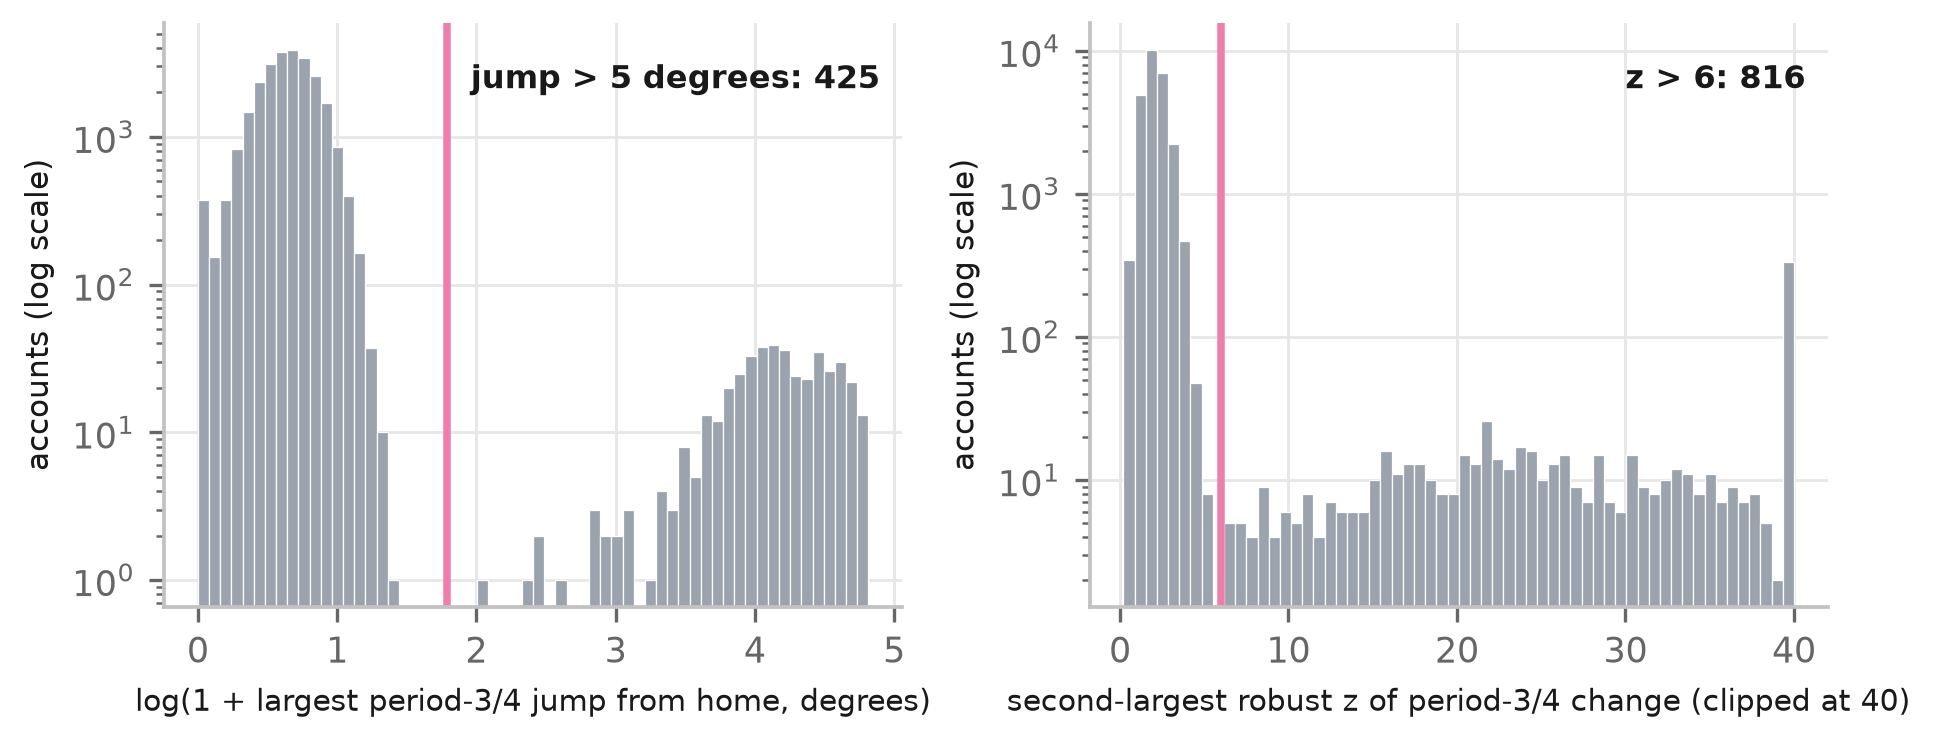
\includegraphics[width=\linewidth]{fig_t5_shock.png}
\caption{Left: largest login-position jump in periods 3/4 (log scale). Right: second-largest robust $z$ of the period-3/4 change across metrics. Both have an empty band between the normal bulk and a long tail of shocked accounts.}
\label{fig:t5-shock}
\end{figure}

In Figure~\ref{fig:t5-shock}, normal accounts stay within about 3 degrees of home and have $z_2<4$. A separate population jumps by more than 5 degrees (425 accounts) or moves at least two metrics at once with $z_2>6$ (816 accounts); a few accounts also report an impossible latitude ($|\text{lat}|>90$). We cut inside the empty band, and the three conditions together flag 827 accounts. The security flags are not used to decide, but they confirm the population: \feat{password_changed}, \feat{vpn_usage} and \feat{mass_item_sale} are enriched almost only inside this group.

\paragraph{Stationary clusters.} A bot or a dormant account does not change over time, so period-to-period change cannot find it. We scanned the four-period mean of every metric and every static feature for a histogram with an empty gap.

\begin{figure}[H]
\centering
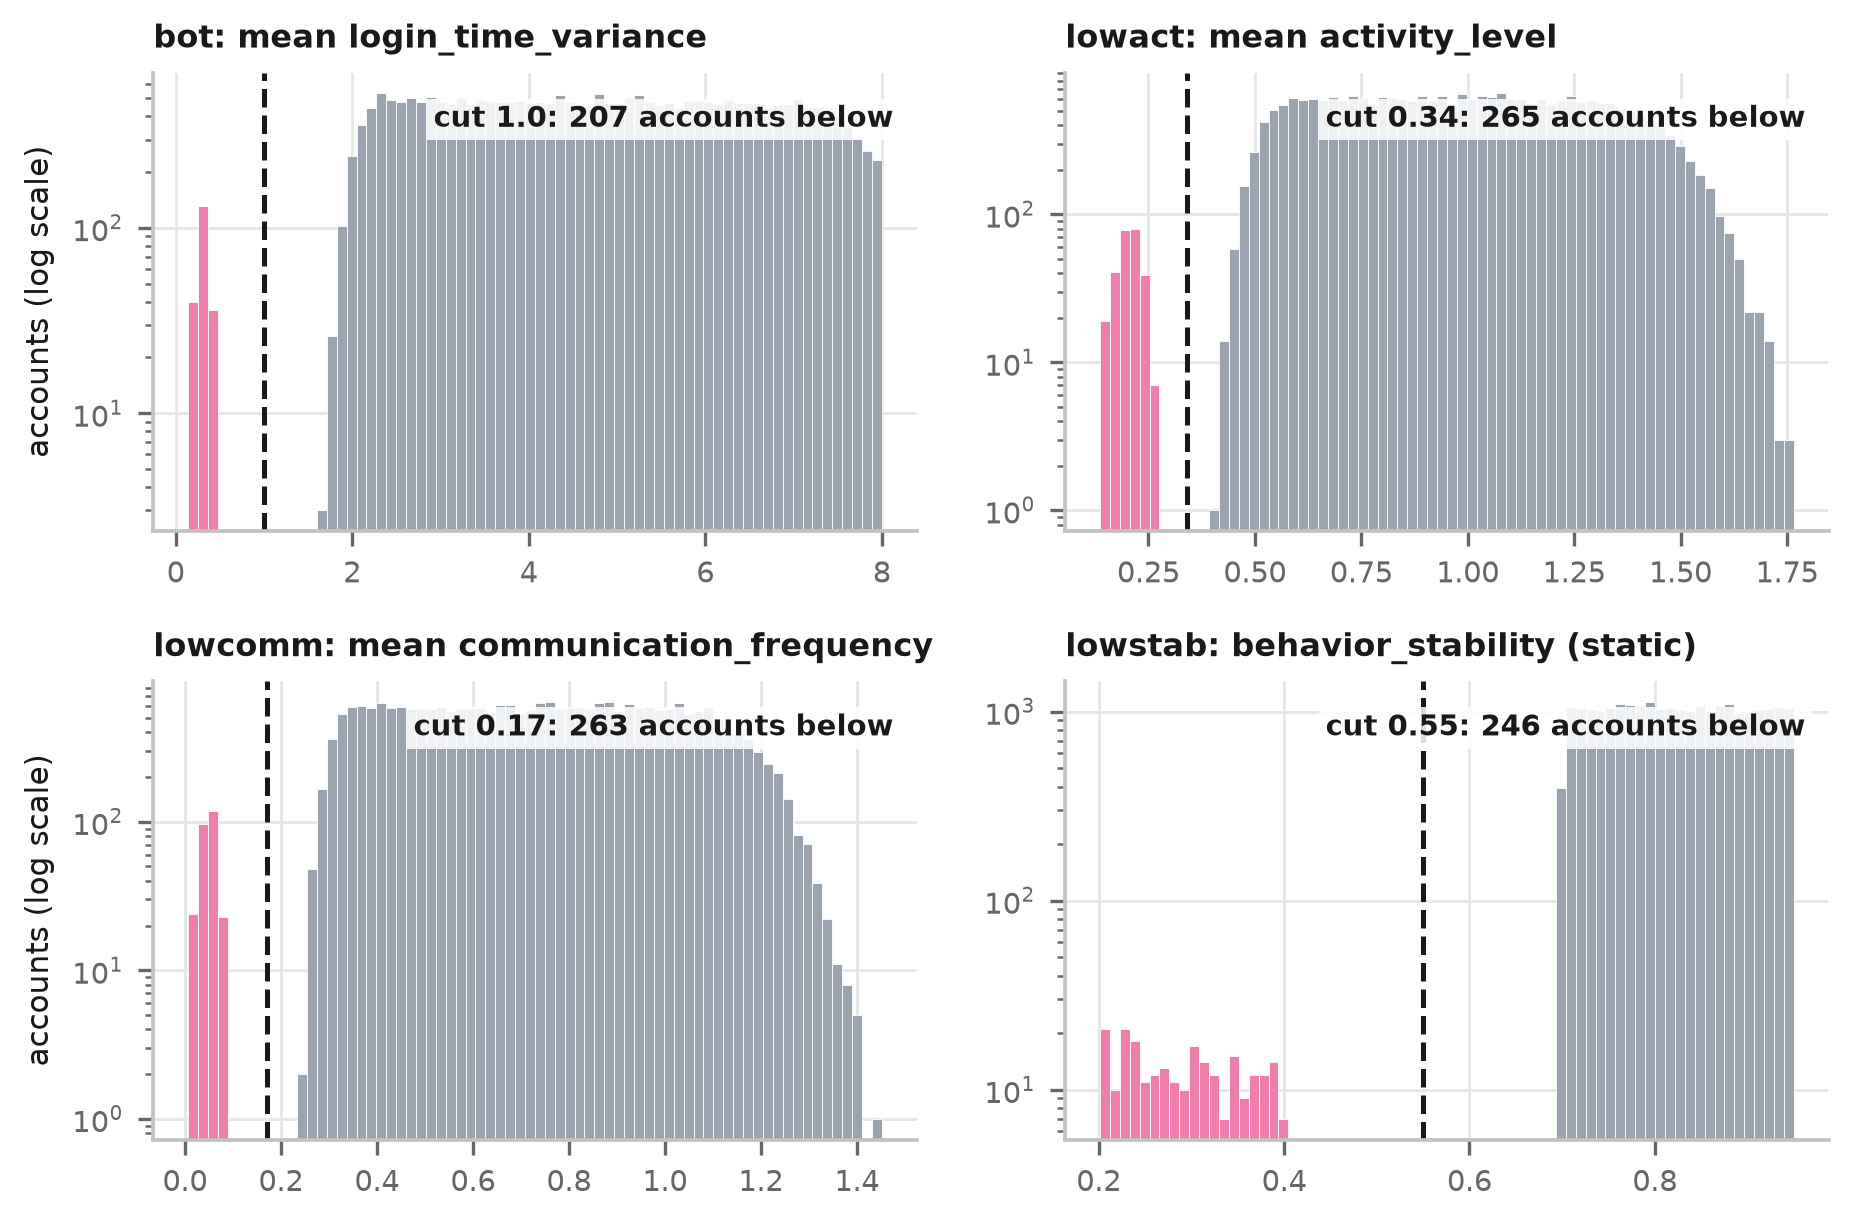
\includegraphics[width=\linewidth]{fig_t5_gaps.png}
\caption{Four features whose histograms (log scale) contain an empty gap between a small anomalous cluster (magenta) and the normal bulk (grey). Dashed line: cut inside the gap.}
\label{fig:t5-gaps}
\end{figure}

Figure~\ref{fig:t5-gaps} shows four such features. In each, no account lies inside the gap we checked (0.5 to 1.5 for \feat{login_time_variance}, 0.30 to 0.40 for \feat{activity_level}, 0.12 to 0.22 for \feat{communication_frequency}, 0.45 to 0.60 for \feat{behavior_stability}), so the exact cut position does not matter. The clusters hold 207, 265, 263 and 246 accounts; we call them \feat{bot}, \feat{lowact}, \feat{lowcomm} and \feat{lowstab}. A full scan of every other mean, standard deviation and static feature found no further isolated cluster.

\paragraph{A box that no single feature shows.} A fifth stationary type hides inside the normal range of every individual feature. It appears only when three statistics are examined together: at all four periods, \feat{performance_stability} lies in $[0.85,0.95]$, \feat{kda_std} in $[0.70,1.00]$ and \feat{accuracy_std} in $[9,12]$.

\begin{figure}[H]
\centering
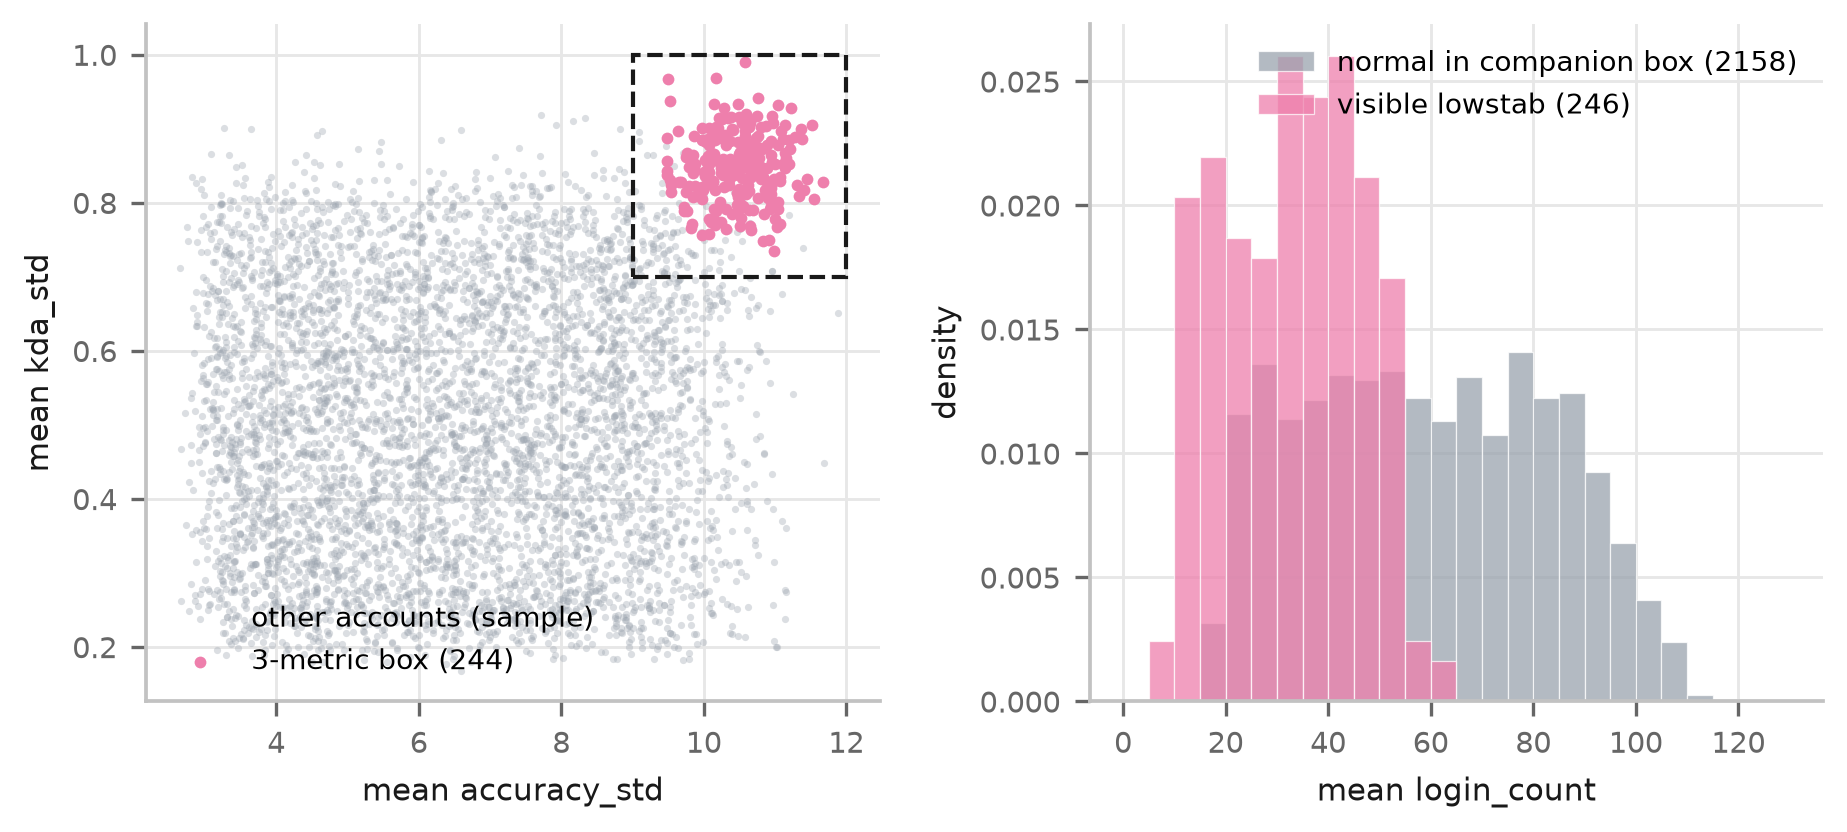
\includegraphics[width=\linewidth]{fig_t5_box_recovery.png}
\caption{Left: the 3-metric box (dashed) contains 244 accounts outside the earlier detectors; a sample of other accounts spreads over the whole plane (the third metric, \texttt{performance\_stability}, is not drawn). Right: accounts with the \texttt{lowstab} pattern have a different mean \texttt{login\_count} than normal accounts inside the same companion box, which is the signal used to recover hidden members.}
\label{fig:t5-box}
\end{figure}

In the left panel of Figure~\ref{fig:t5-box}, the 244 accounts of the box form a tight clump in a corner of the plane that no one-dimensional histogram can show. In the right panel, accounts with a visible low \feat{behavior_stability} also share a narrow range of \feat{purchase_frequency} (3 to 6) and of \feat{account_age_days} (800 to 1,500); inside that companion box their mean \feat{login_count} is lower than that of normal accounts. This matters for the 4.86\% of accounts whose \feat{behavior_stability} is missing: the cluster cut cannot test them, so some anomalies must hide there (about 14 expected, since $246\times0.0486/(1-0.0486)\approx 12.6$).

\paragraph{Remaining structure.} A local analysis of the new file (not part of the submission notebook) found that the median $|r|$ between feature pairs is 0.0049 with a maximum of 0.24 over all accounts, but 0.0044 and 0.026 for the 23,785 accounts that are not flagged. The correlation in the full file therefore came from the anomalies, and the normal accounts are close to independent, which is why we expect nothing structured to be left for a further detector. The same analysis counts 18 anomalies hidden behind missing cells, which is the target of the recovery step below.

\subsubsection{Data Preprocessing}

There is no train set, so preprocessing consists of per-account summaries that make each anomaly type visible, computed from the test file only. Table~\ref{tab:t5-evidence} links each figure to the decision it motivated.

\begin{evidencetable}{EDA evidence and the pipeline decision it motivated (task 5).}{tab:t5-evidence}
Figure~\ref{fig:t5-shock}. Normal accounts stay near home and change little; a separate tail jumps $>5^\circ$ or moves $\ge2$ metrics with $z_2>6$ & Rule detector on periods 3/4 versus the baseline of periods 1/2, cut inside the empty band. \\
Figure~\ref{fig:t5-gaps}. Four features have empty gaps that isolate small clusters & Exact gap cuts per cluster (\feat{bot}, \feat{lowact}, \feat{lowcomm}, \feat{lowstab}) instead of one black-box anomaly score. \\
Figure~\ref{fig:t5-box} (left). A fifth type hides in a joint box of three metrics at all four periods & Box detector on \feat{performance_stability}, \feat{kda_std} and \feat{accuracy_std}. \\
Figure~\ref{fig:t5-box} (right). Hidden members have a distinct \feat{login_count} inside their companion box & Bayesian posterior for accounts with missing \feat{behavior_stability}, flagged above $p>0.10$ (the break-even of $F_3$). \\
\end{evidencetable}

\paragraph{Features.} Four summaries are used. (i) The \emph{home position} is the mean of the period-1 and period-2 login coordinates. (ii) The \emph{period change} of a metric is the largest absolute difference between its period-3/4 values and the mean of its period-1/2 values; its robust $z$-score uses the median and $1.4826\times$MAD of the change over all accounts. (iii) The \emph{four-period mean} of a metric detects stationary clusters. (iv) The four-period mean of \feat{login_count} and the period-wise standard deviation of \feat{purchase_frequency} feed the recovery step.

\paragraph{Missing values.} Missing cells are \emph{not imputed}. The geo and shock rules use NaN-aware means and maxima. The box detector treats a missing cell as compatible with the box: an account fails only if an observed value falls outside it. Missingness is modelled in one place only, the recovery of hidden \feat{lowstab} accounts. Invalid latitudes (absolute value above 90) are flagged and masked out of the distance computation.

\subsubsection{Model Design}
\label{sec:t5-model}

The final detector is a union of four unsupervised components. Figure~\ref{fig:t5-pipeline} shows the flow and Table~\ref{tab:t5-detectors} lists each detector, its rule and its size. All of them are density or histogram-based: the rules use robust $z$-scores (a median/MAD test of how far a change lies outside the bulk), and the gap and box detectors flag regions of feature space that are empty in the bulk of the data. This is anomaly detection in the sense of the course (find points where the density is abnormally low), implemented with explicit one-, two- and three-dimensional regions instead of a generic score.

\begin{figure}[H]
\centering
\begin{tikzpicture}[x=1cm,y=1cm]
\node[stage] (raw) at (0,0) {Test file\\25,889 accounts, 123 columns, no labels};
\node[stage,fill=\taskcolor{5}!12] (feat) at (5.4,0) {Per-account summaries\\home position, period change and robust $z$, four-period means};
\node[stage] (scan) at (10.8,0) {Empty-gap scan\\every mean, std and static feature};
\node[model,draw=\taskcolor{5}] (A) at (0,-3.4) {\textbf{Shock rule} (827)\\geo jump $>5^\circ$, $|\text{lat}|>90$, or $z_2>6$};
\node[model,draw=\taskcolor{5}] (B) at (5.4,-3.4) {\textbf{Gap clusters} (981)\\bot 207, lowact 265, lowcomm 263, lowstab 246};
\node[model,draw=\taskcolor{5}] (C) at (10.8,-3.4) {\textbf{3-metric box} (244 new)\\all periods in the joint box};
\node[stage,text width=9.6cm] (union) at (5.4,-6.0) {Union of rule, clusters and box: 2,052 accounts};
\node[decision,draw=\taskcolor{5},thick] (rec) at (2.7,-8.4) {Posterior recovery\\missing \feat{behavior_stability}, 129 candidates, $p>0.10$};
\node[stage,fill=\taskcolor{5}!12] (out) at (8.1,-8.4) {Flagged\\2,104 accounts (8.13\%)};
\draw[flow] (raw) -- (feat);
\draw[flow] (feat) -- (scan);
\draw[thick,ink!75] (feat.south) -- (5.4,-1.8);
\draw[thick,ink!75] (0,-1.8) -- (10.8,-1.8);
\draw[flow] (0,-1.8) -- (A.north);
\draw[flow] (5.4,-1.8) -- (B.north);
\draw[flow] (10.8,-1.8) -- (C.north);
\draw[flow] (A.south) -- (A.south |- union.north);
\draw[flow] (B.south) -- (B.south |- union.north);
\draw[flow] (C.south) -- (C.south |- union.north);
\draw[flow] (union.south) -- ++(0,-0.5) -| (rec.north);
\draw[flow] (rec) -- node[above,font=\scriptsize]{+52} (out);
\draw[flow] (union.south) -- ++(0,-0.5) -| (out.north);
\node[note,anchor=north] at (5.4,-9.9) {no labels: cuts sit in empty gaps; the recovery threshold is the $F_3$ break-even};
\end{tikzpicture}
\caption{Task 5 pipeline: three detector families on one test file, a union, and a Bayesian recovery of accounts hidden by missing values.}
\label{fig:t5-pipeline}
\end{figure}

\begin{table}[H]\centering\small
\caption{Detectors, decision rules and the number of accounts each contributes.}\label{tab:t5-detectors}
\begin{tabular}{@{}L{.20\linewidth}L{.58\linewidth}r@{}}
\toprule
\textbf{Detector} & \textbf{Rule} & \textbf{Accounts} \\
\midrule
Shock rule & geo jump of periods 3/4 $>5^\circ$ from home, or $|\text{lat}|>90$, or $\ge2$ metrics with robust $z>6$ & 827 \\
\feat{bot} & mean \feat{login_time_variance} $<1.0$ & 207 \\
\feat{lowact} & mean \feat{activity_level} $<0.34$ & 265 \\
\feat{lowcomm} & mean \feat{communication_frequency} $<0.17$ & 263 \\
\feat{lowstab} & \feat{behavior_stability} $<0.55$ & 246 \\
Union of the five rows above & overlaps counted once & 1,808 \\
3-metric box & periods 1 to 4 inside the three intervals of Figure~\ref{fig:t5-box}; missing cells allowed & 244 new \\
Posterior recovery & \feat{behavior_stability} missing, not yet flagged, inside the companion box, posterior $>0.10$ & 52 new \\
\midrule
\textbf{Final} & & \textbf{2,104} \\
\bottomrule
\end{tabular}
\end{table}

\paragraph{Rule detector.} The $z$-score is robust because the median and MAD are not moved by the anomalies themselves. Requiring two metrics at once suppresses a single noisy column, and the geo and latitude conditions catch takeovers that move the login location without a large change in behaviour. The cut sits in the empty band of Figure~\ref{fig:t5-shock}; widening it ($z\in[4,6]$, $2^\circ$ to $5^\circ$) added 356 accounts and lowered the public score by 0.0025 (Section~\ref{sec:t5-failed}).

\paragraph{Gap clusters and box.} Each cluster test is a threshold on a four-period mean (or on the static feature) placed in the middle of an empty gap. The box detector is the same idea in three dimensions, with every period required to fall inside the box. Because these regions are read from where the data are empty and not fitted to a distribution, we expected them to carry over to a re-generated file, and they did (Section~\ref{sec:t5-eval}).

\paragraph{Bayesian recovery of hidden low-stability accounts.} Accounts with a missing \feat{behavior_stability} cannot be tested against the 0.55 cut. We keep those outside the union that lie in the companion box (\feat{purchase_frequency} in $[3,6]$ at all periods, \feat{account_age_days} in $[800,1500]$): 129 candidates. For each we compute a log-likelihood ratio from two histogram densities, $\log f_{\text{lowstab}}/f_{\text{normal}}$, of the four-period mean of \feat{login_count} (26 bins on $[0,130]$) and of the standard deviation of \feat{purchase_frequency} (25 bins on $[0,2.5]$). The visible \feat{lowstab} accounts give $f_{\text{lowstab}}$, and normal accounts in the same box (\feat{behavior_stability} $\ge0.6$) give $f_{\text{normal}}$. With a prior of 14 hidden members among the candidates, the posterior is the logistic function of the ratio plus the log prior odds. We flag $p>0.10$, the break-even derived in Problem and Data; this flags 53 accounts, of which 52 are new.

\subsubsection{Evaluation and Results}
\label{sec:t5-eval}

\paragraph{Validation without labels.} There is no OOF score. We use three kinds of evidence instead. (i) \emph{Structure}: each detector is an empty gap or a joint box, so its precision is high by construction, and the unflagged accounts show no leftover structure. (ii) \emph{Isolated public-leaderboard probes}: a submission that changes only the Task 5 column measures the change of Task 5 alone ($\Delta\text{LB}\approx 0.2\,\Delta F_3$). Figure~\ref{fig:t5-decision-log} lists every probe. (iii) \emph{Transfer across the data re-release}: the 12 November release regenerated every row; the same code, without retuning, found clusters of the same sizes in the new file (207, 265, 263 and 246 accounts, and a box of 244).

\begin{figure}[H]
\centering
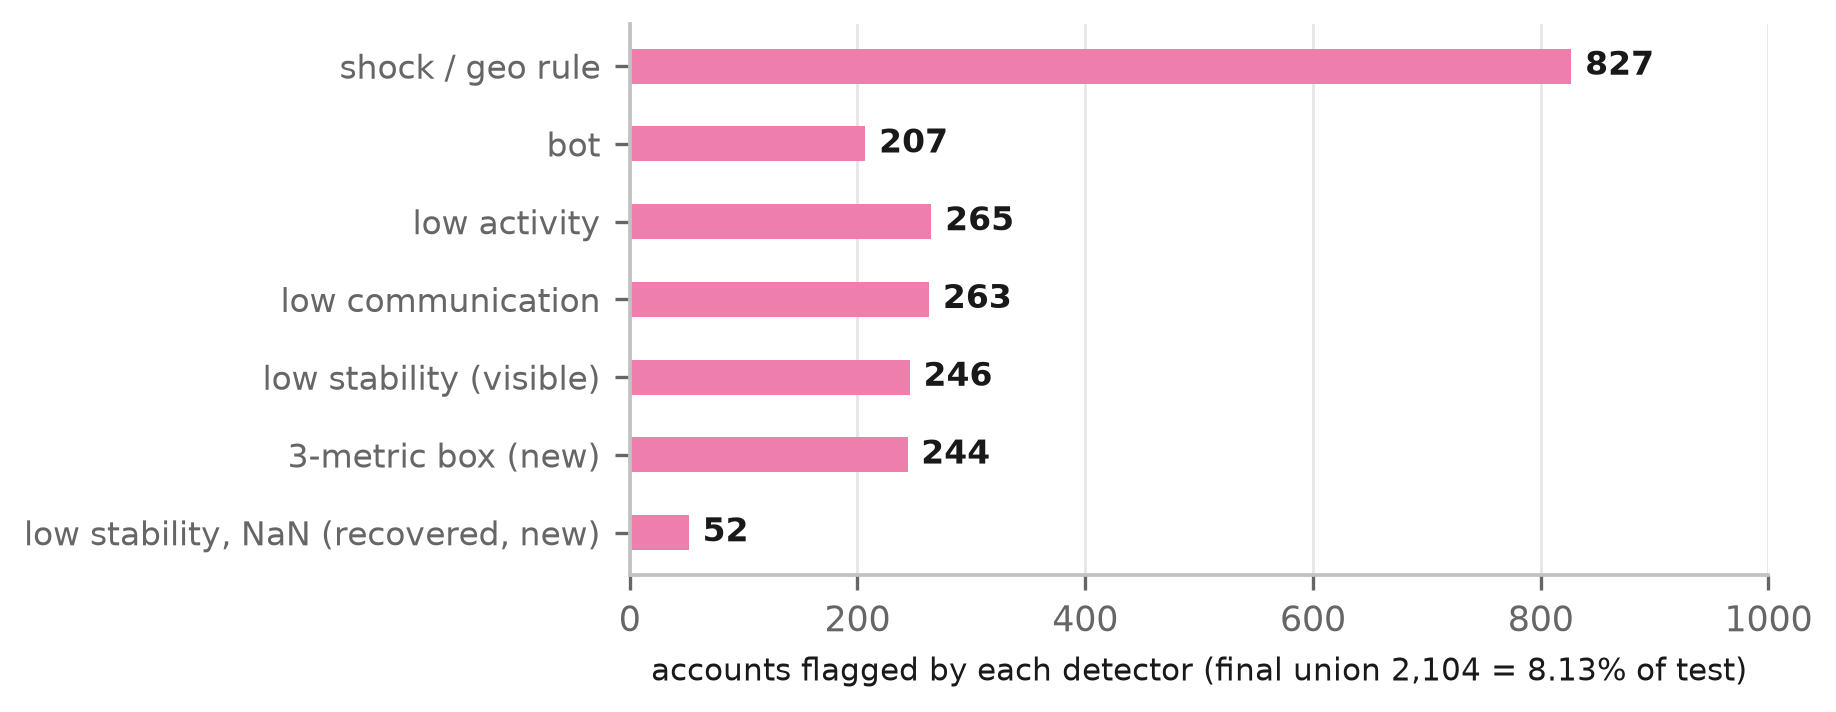
\includegraphics[width=\linewidth]{fig_t5_breakdown.png}
\caption{Accounts flagged by each detector on the 12 November test file. The shock rule and the clusters partly overlap; the last two bars are the accounts that the box detector and the recovery step add to the earlier union.}
\label{fig:t5-breakdown}
\end{figure}

Figure~\ref{fig:t5-breakdown} and Table~\ref{tab:t5-results} summarise the final file.

\begin{table}[H]\centering\small
\caption{Result summary for Task 5. No labelled score exists; leaderboard quantities are inferred from isolated probes and the F3 value is an estimate.}\label{tab:t5-results}
\begin{tabular}{@{}L{.50\linewidth}L{.42\linewidth}@{}}
\toprule
\textbf{Quantity} & \textbf{Value} \\
\midrule
Flagged accounts & 2,104 of 25,889 (8.13\%) \\
Weight of Task 5 in the public score & about 0.2 (all-zero column: $-0.177$) \\
Estimated F3 of this file (hidden-member accounting) & 0.99681 \\
Same estimate with the best-known extra hidden rows (2,115 flagged) & 0.99698 \\
Leaderboard effect of the last tested changes & between $-0.00025$ and $+0.00002$ \\
\bottomrule
\end{tabular}
\end{table}

\paragraph{How close to complete the file is.} The estimate of 0.9968 comes from an accounting of the generator, not from labels. The file flags every visible anomaly group. The remaining error is the part hidden behind missing values: 18 anomalies (one \feat{lowact} account whose activity is missing at all four periods, and about 17 \feat{lowstab} accounts with a missing \feat{behavior_stability}), of which the recovery step catches some. An alternative file with 2,115 rows (the \feat{lowact} account and a prior of 17) has an estimated F3 of 0.99698; submitted, its 11 extra rows scored $-0.0001$, below the resolution of the public leaderboard, so we kept the 2,104-row file.

\paragraph{Decision log.} Figure~\ref{fig:t5-decision-log} shows every Task 5 experiment in our log. Each delta is relative to the best submission at the time. The first row shows the weight of the task; the box detector was the one large kept gain (an estimate, because the submission that introduced it also changed other tasks); every later experiment was noise or a loss.

\begin{figure}[H]
\centering
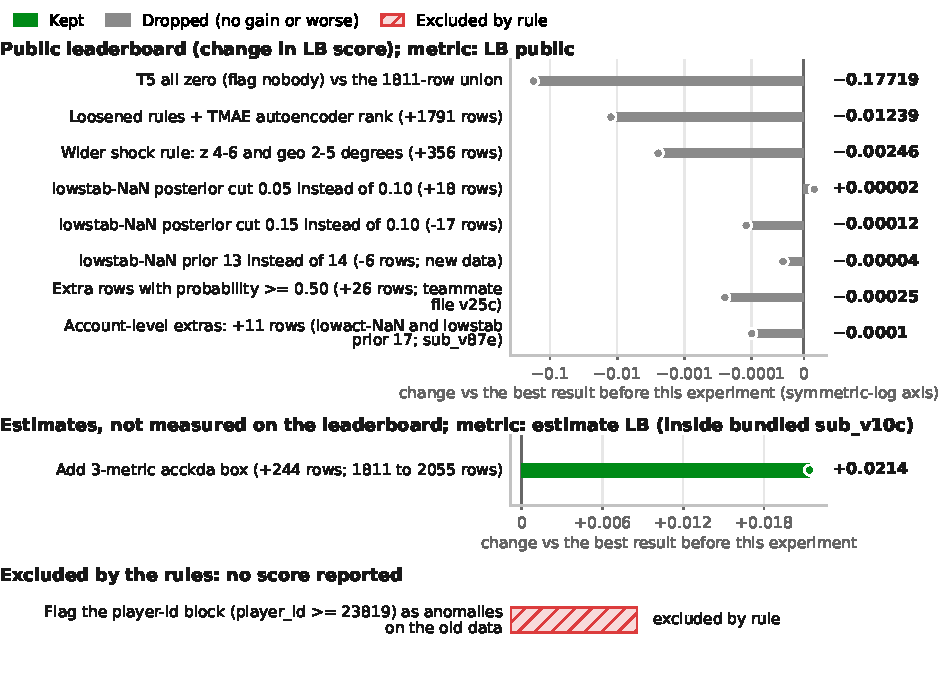
\includegraphics[width=\linewidth,height=0.72\textheight,keepaspectratio]{decision_log_t5.pdf}
\caption{Task 5 decision log. Grey bars: experiments we dropped; green: the kept experiment; hatched red: a leak shortcut excluded by the rules. The public-leaderboard panel uses a symmetric-log axis because the all-zero probe is more than a thousand times larger than the last changes.}
\label{fig:t5-decision-log}
\end{figure}

\subsubsection{Insights from Model Behaviour}

\paragraph{What the detectors found.} The anomalies have the structure of an explicit generator. The shock group splits into three kinds (takeover 310, account selling 310, VPN abuse 207), the bot group has 207 accounts, and the stationary anomalies are four boxes of 244 to 265 accounts. Together they are about 8\% of the file. In the first data release the same anomalies sat in a block of consecutive \feat{player_id} values; the re-release removed that, and our detectors found groups of the same size without using the id.

\paragraph{Why simple detectors beat a general anomaly score.} A stationary anomaly deviates in only one to three of more than 100 features. An isolation tree or a reconstruction error is sensitive to all features at once, so a deviation in one feature inside the normal marginal range is diluted. Table~\ref{tab:t5-baselines} shows the effect: Isolation Forest finds the extreme tails but only 10\% to 32\% of the stationary groups, and the autoencoder is worse.

\paragraph{Where the detector is weakest.} Hidden members behind missing values are the only systematic error. Under the recall-heavy metric we flag 53 of the 129 candidates although only about 17 anomalies are expected among them: each wrong flag adds one unit to the denominator, whereas each missed anomaly adds nine.

\paragraph{Robustness to data re-generation.} The pipeline was written on the first release and transferred to the second without changing any cut. Rules placed in empty gaps are stable under resampling; rules placed inside a dense distribution would not be.

\subsubsection{Common Mistakes and Failed Experiments}
\label{sec:t5-failed}

\paragraph{Adding rows beyond the union costs score, every time.} Every change that flagged more accounts lowered the public score. A loosened rule set plus the top-ranked accounts of an autoencoder added 1,791 rows and cost $-0.0124$; widening the shock cut added 356 rows ($-0.0025$); a teammate's probability cut at 0.50 added 26 rows ($-0.00025$); our own recovery extras added 11 rows ($-0.0001$). The added accounts held about 0\% to 5\% true anomalies, far below the roughly 10\% break-even of the metric.

\paragraph{Black-box detectors do not fit this problem.} The course brief names Isolation Forest and autoencoders, so we tested them (Table~\ref{tab:t5-baselines}). They find extreme tails but cannot place a cut: with no labels, a percentile cut-off is a guess, whereas empty gaps give a clean one. The values come from our local research notes and measure agreement with the union we found, not with the hidden truth, so they show what each method misses and not its true recall.

\begin{table}[H]\centering\small
\caption{Standard anomaly detectors compared with the final union. Agreement is the share of a group inside the detector's top 2,104 accounts (new data), or ROC-AUC against the first release's 1,811-row union (first data).}\label{tab:t5-baselines}
\begin{tabular}{@{}L{.27\linewidth}L{.12\linewidth}L{.55\linewidth}@{}}
\toprule
\textbf{Method} & \textbf{Data} & \textbf{Result} \\
\midrule
Isolation Forest (500 trees, top 2,104) & new & takeover 99.4\%; selling, VPN and bot 100\%; lowact 12.8\%, lowcomm 17.9\%, lowstab 31.7\%, 3-metric box 10.2\%, hidden 0\%; 888 flagged accounts (42.2\%) outside the final set \\
Temporal masked autoencoder (3-layer Transformer, top 2,104) & new & takeover 55.2\%, selling 6.1\%, VPN 32.8\%, bot 5.8\%, stationary groups 5.3\% to 10.2\%, hidden 15.4\%; 1,743 accounts (82.8\%) outside the final set \\
One-class SVM, Mahalanobis distance, PCA reconstruction, Gaussian mixture, LOF & first & AUC 0.86, 0.87, 0.80, 0.80 and 0.52 \\
\bottomrule
\end{tabular}
\end{table}

\paragraph{The autoencoder.} The temporal masked autoencoder separated our rule set (AUC 0.83) but not the full union (AUC 0.66), so adding its top-ranked accounts only added normal accounts, and the submission that did so is the $-0.0124$ row above. We did not use it.

\paragraph{A leak we did not use.} In the first release the anomalous accounts occupied a contiguous block of \feat{player_id} (identifiers 23,819 and above, 2,070 accounts). Flagging that block matched our box set almost exactly. It is not a behavioural signal, and every clean submission and every number in this section uses behaviour only. The re-release removed the block (AUC of the id against our flags is 0.50). The team's rule status for a Task 5 pipeline whose thresholds are necessarily read from the unlabeled test file (there is no train set) is \todo{confirm with the TA that gap and box cuts read from the test file are allowed for Task 5}.

\paragraph{Tuning on a few rows.} Moving the recovery threshold from 0.10 to 0.05 gave $+0.00002$, to 0.15 gave $-0.00012$, and changing the prior from 14 to 13 gave $-0.00004$. These are changes of a few rows and cannot be distinguished from noise, so we kept the break-even threshold and stopped tuning.

\subsubsection{Domain Interpretation and Business Impact}

The detector flags 8.13\% of accounts. For a security team that is drowning in alerts, the useful output is the \emph{type} of each flag: takeover candidates (location jump with several metrics moving), account-selling or VPN candidates, bot farms (very low \feat{login_time_variance}), and dormant or scripted accounts (low activity, low communication, low stability, or the 3-metric box). Each type needs a different response, so a production system should report why an account was flagged and not only a score. This explainability is a direct advantage of the rule-based design over a black-box score.

The metric reflects a realistic cost structure: a missed takeover or selling ring costs far more than a manual review. Under $F_3$ the break-even probability is about 10\%, so an account should go to review when it is at least about 10\% likely to be anomalous. In production this is a tunable threshold that should follow the review team's capacity and the cost per false alarm.

\paragraph{Caveats for deployment.} The empty gaps in Figure~\ref{fig:t5-gaps} come from the synthetic generator. Real traffic has no clean gaps, and we could not measure the precision of a flag without labels. We would keep these detectors as a transparent baseline, add an isolation-forest or autoencoder model trained on real traffic and calibrated on analyst feedback, and use rolling windows so that a legitimate traveller or a rapidly improving player is not flagged indefinitely.

\end{document}
